\chapter{显微成像系统整体方案设计}
本显微成像检测系统由光学模块、图像处理模块、图像采集模块、图像归档显示模块等构成。在整体设计流程中,关键的技术包括图像传感器的分析与选择、图像主处理器及预处理器的选择等。本章在光学基础上,根据需求和情境重点分析了各个不同模块需要的硬件优势方面和选型,并对此进行较为详细的讲述。可见的一个分类的图\ref{fig:module_1}示如:
\begin{figure}[h]
\centering
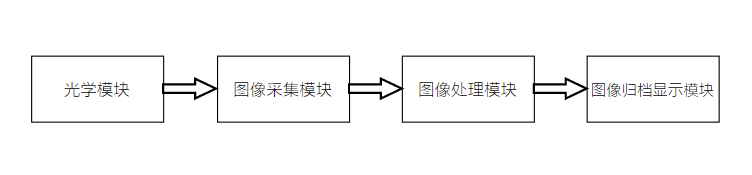
\includegraphics[width=0.7\linewidth]{Figure/module_1}
\caption{模块介绍}
\label{fig:module_1}
\end{figure}


\section{显微基本原理}
\subsection{光学成像原理}

显微镜的成像如图\ref{fig:micro_1}所示,小物体AB在物镜的焦距之外,人眼在另一边的距离除观察,AB形成放大倒立的实像A'B',而这一实像正好在目镜的焦距以内的附近处,再一次经过目镜放大之后,在明视距离d处形成正立虚像A"B"\cite{lightxidian}。


\begin{figure}[h]
	\centering
	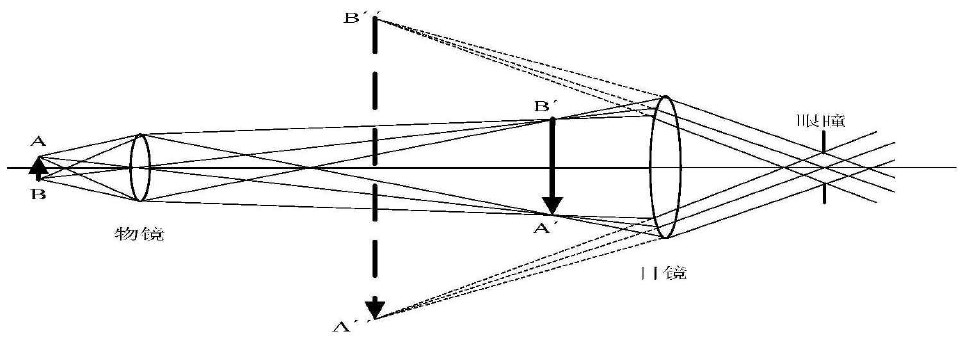
\includegraphics[width=0.7\linewidth]{Figure/micro_1}
	\caption[显微镜成像光路图]{显微镜成像光路图}
	%\caption{显微镜成像光路图}
	\label{fig:micro_1}
\end{figure}

显微镜的视觉放大率定义为:

\begin{equation}
\label{j2}
J = l_{0}\cdot d / f_{1}f_{2}
\end{equation}

式\ref{j2}中 $d$ 是明视距离,$l_{0}$为物镜到目镜的距离, $f_{1}$ 为物镜的焦距, $f_{2}$ 为目镜的焦距。此处的角放大率为物镜的线放大率和目镜的角放大率的乘积。
数值孔径的孔径角的正弦与透镜和物体之间介质的折射率的乘积,而显微镜的分辨率与光的波长和物镜的数值孔径有关,波长越短,数值孔径越大,分辨率越大\cite{fenbianlv}。


\subsection{显微镜结构构造}
普通光学显微镜的构造可分为两部分:一为机械装置,一为光学系统 。机械装置由镜座、镜筒、物镜转换器、载物台、推动器、粗动螺旋和微动螺旋等部件组成。光学系统由目镜、物镜、聚光器、光源、滤光片、虹彩光圈等组成。
一个典型显微镜如图\ref{fig:mi_1}所示。
\begin{figure}[h]
\centering
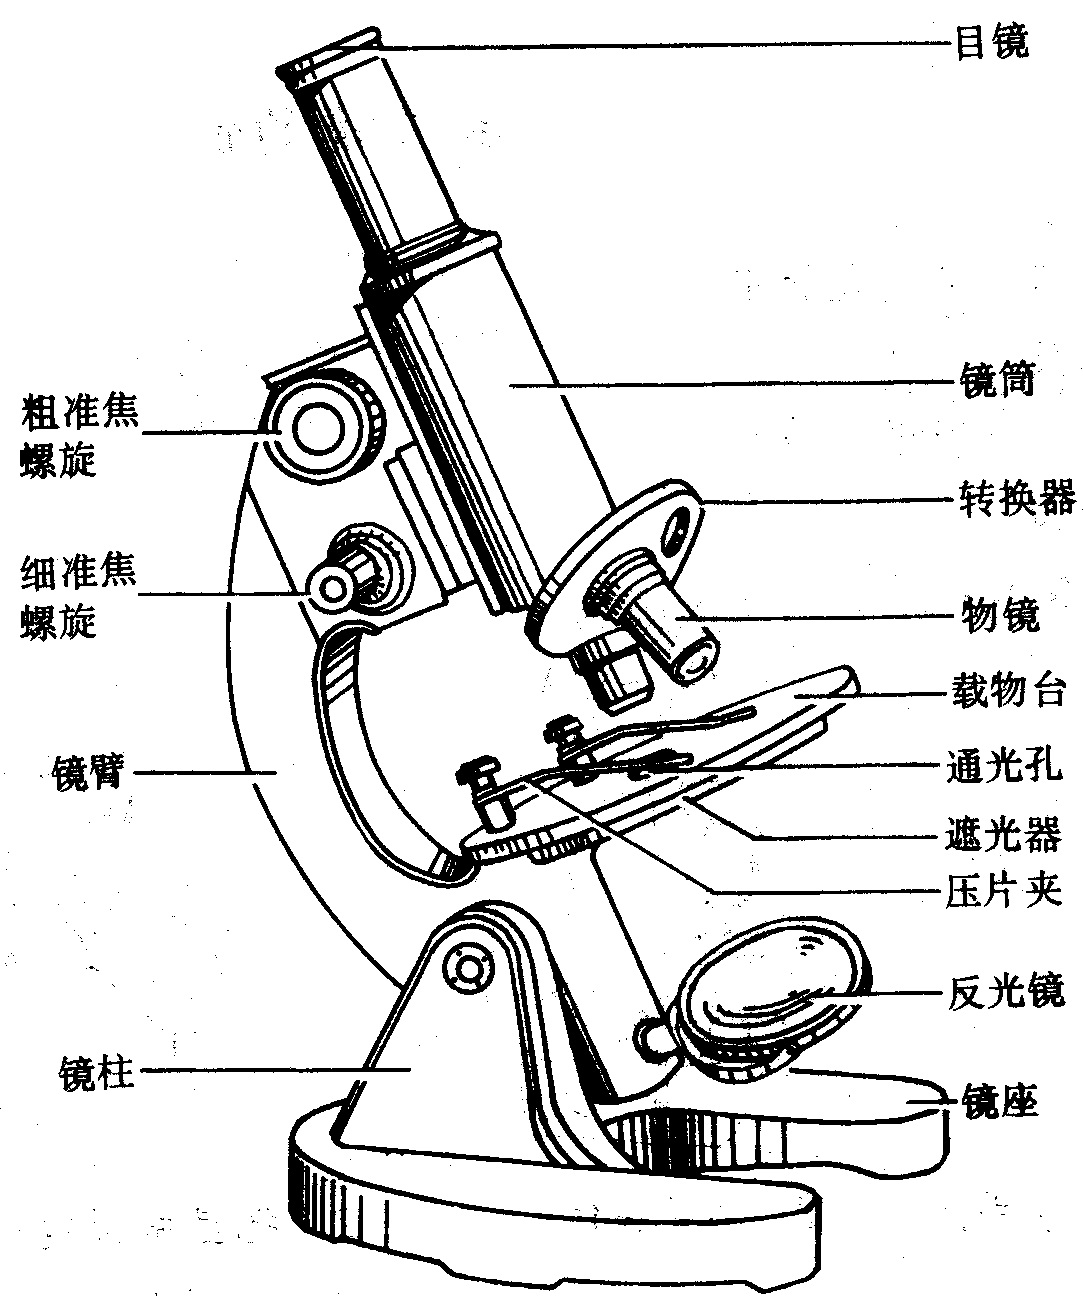
\includegraphics[width=0.5\linewidth]{Figure/mi_1}
\caption{典型显微镜结构图}
\label{fig:mi_1}
\end{figure}


物镜是决定显微镜性能的最重要部件,安装在物镜转换器上,接近被观察的物体,故叫做物镜或接物镜。通常目镜由上下两组透镜组成,上面的透镜叫做接目透镜,下面的透镜叫做会聚透镜或场镜。聚光器也叫集光器。位于标本下方的聚光器支架上。它主要由聚光镜和可变光阑组成。其中,聚光镜可分为明视场聚光镜和暗视场聚光镜。反光镜是一个可以随意转动的双面镜,直径为50mm,一面为平面,一面为凹面,其作用是将从任何方向射来的光线经通光孔反射。平面镜上反射光线的能力较弱,适合在光线较强时使用,凹面镜反射光线的能力较强,适合在光线较弱时使用。

\section{显微成像处理平台器件选型}
\subsection{显微镜头物镜选型}
常见的物镜通过像差校正程度的不同,可划分为:消色差物镜、复消色差物镜,半复消色差物镜和特种物镜。这里选用最简单的消色差物镜,通过减少透镜的片数降低选择的难度。

下面对物镜中常见的一些重要的参数和公式做出解释。

物镜的数值孔径:
\begin{equation}
\label{NA}
\mathit{NA} = n\sin \alpha 
\end{equation}

式\ref{NA}中,$\alpha$代表物镜在物方的孔径半角,$n$ 表示物空间的介质折射率。增加数值孔径的方式可以通过增加透镜的孔径或者采用焦距较短的物镜来增大孔径半角$\alpha$。

两物镜的最小分辨距离表现为:
\begin{equation}
\label{one}
\mathit{K}\lambda / n\sin \alpha 
\end{equation}

在式\ref{one}中, $\lambda$为成像光线的波长,$n$为测试物周围物质的折射率, $\mathit{K}$为数值, 由式\ref{NA}可知,$n\sin \alpha$即$\mathit{NA}$常表示为物镜的数值孔径。数值孔径越大,能够分辨两物点的最短距离则越小,分辨率越高。

\begin{equation}
\label{dd}
d/f \approx  1.22/D
\end{equation}
\begin{equation}
\label{nd}
ndsin \alpha=n'd'sin \alpha'
\end{equation}


式\ref{dd}中,,考虑到实际因素,考虑式\ref{nd}条件,其中$n$为物空间折射率,$n'$为像空间折射率,在空气介质中,取 $\alpha'$为 1;$\alpha$ 是光线在物空间的孔径角,$\alpha'$是对应的像空间共轭点的孔径角;$d$ 为物平面上两点的 间距,$d'$为像面上两像点中心间距,$f$ 为透镜的焦距。考虑到斜入射光线的影响,修正 后的公式表示为:$d=0.5/NA$,其中 $nsin\alpha$ 即物镜的数值孔径。 

通过减小对饮照明光的波长和增大数值孔径的方式可以提高物镜的分辨能力,通常试验中使用波长较短的黄绿光提升分辨能力。

在物镜的放大倍率上,通常为人眼明视距离处的分辨出0.15到0.30mm大小,一般认为是0.20mm。如果过小的话,将不能良好分辨。

最后的设计为物镜的放大倍数为10,光源的照明波长认定为550nm,透镜数值孔径由式\ref{NA}测得为0.6。最后判定物镜的焦距大致范围,便于物镜选型和后期的进一步微调。

\subsection{图像传感器的选型}
固体图像传感器已经广泛地应用于生活各处,包括像电子照相机、DV、智能监控、手机、平板和摄像头等。固体图像传感器是利用半导体材料的内光电效应原理制成的光电转换器件,依据工艺结构可以分为两大类:一类是电荷耦合器件(CCD)图像传感器;另一类是互补金属氧化物(CMOS)图像传感器。两种目前常见的图像传感器都是上世纪60年代开始研制,在当时由于CCD图像传感器灵敏度更高、噪声较低而成为当时图像传感器的主流。而CMOS图像传感器由于工艺上的提升限制,长时间未能摆脱光照灵敏度低、噪声无法下降和图像分辨率低等不足。于此同时,CCD图像传感器由于敏感元件和信号处理电路无法集成在同一芯片上,使得照相机体积大、功耗大\cite{CCDCMOSf}。

进入新世纪,时间发展,随着互联网向移动互联网的转移,智能手机的发展十分迅速,由于CMOS图像传感器却有集成度高、体积小、功耗小和造价低等优点,十分适合在手机上进行集成,考虑到两种图像传感器的技术特点和缺点改进方式,随集成电路设计技术和迭代工艺水平的提高,CMOS图像传感器过去存在的缺点,现在开始逐渐进行技术攻关,常见的背照式结构让CMOS图像传感器在光线摄入上有长足的发展,而且它其固有的特点更是CCD器件所无法比拟的,因而它再次成为研究和工业需求的热点。

\begin{figure}[h]
\centering
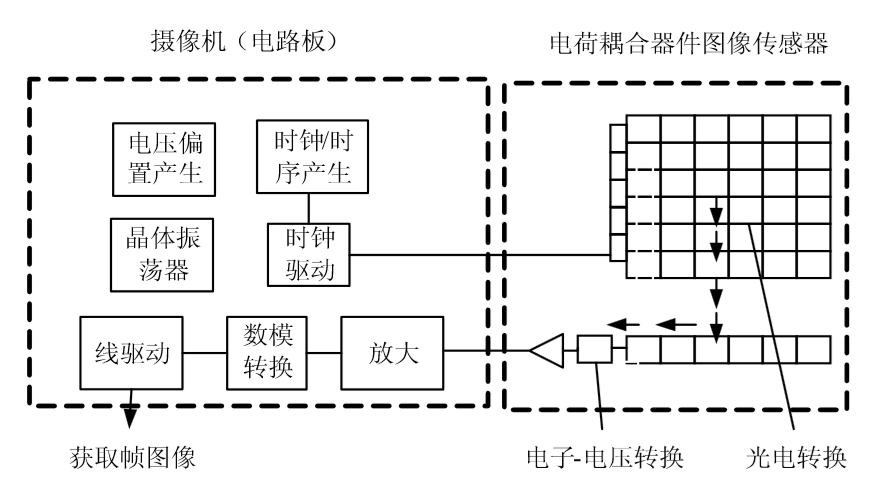
\includegraphics[width=0.7\linewidth]{Figure/CCD_1}
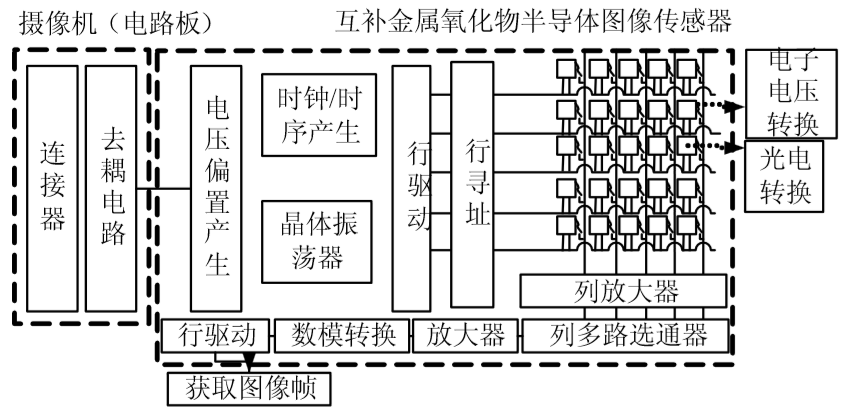
\includegraphics[width=0.7\linewidth]{Figure/CMOS_1}
\caption{}
\label{fig:CCD_1}
\end{figure}

\subsubsection{CMOS和CCD的比较}
CCD和CMOS两者在多个维度上有着较大特性上的差异:

1.系统集成 \\

CMOS图像传感器易于在SoC上集成,便于在同一芯片中同时进行内部的信号降噪、数据整合和数据处理,片上数据传输率高,与周边电路的整合性高,更可可将与信号处理器整合在一起,如图所示,便于大幅度减小对应模块的主板面积占用。考虑到 CCD 和 CMOS 两者采用不同的制造工艺,所以 CCD 难以装入SoC。因此,一般认为CMOS图像传感器可以广泛使用在各个嵌入式领域。

2.性能特性\\

在实际应用方面,性能特性是进行芯片选型取舍的极为重要的因素。CMOS图像传感器由于多个放大器的存在,不同一组生产的放大器放大情况有细微差异,导致最终的图像输出噪声较多。此外,由于集成度高的缘故,各元件、电路之间距离较近,相互之间的光、电、磁干扰显得严重,噪声对图像质量影响很大。在需要的电源数方面,相对于CCD图像传感器需要三或四组电源,CMOS图像传感器则只需一个即可。
而且CMOS图像传感器利用3.3V电源即可驱动,相比之下电源消耗量比CCD图像传感器低。因此,在功耗和电压方面,CMOS图像传感器比CCD图像传感器在小型化嵌入式设备中有更大的优势。此外,CMOS信号读取的方式较为简易,电路设计相应也可简单。

3.可靠性\\

两种图像传感器在商用及工业应用领域具有等价的可靠性。在极端恶劣的应用环境中,由于CMOS图像传感器充分提高系统集成度、降低模块间耦合,借助设计良好的封装和焊接技术,其可靠性优于CCD图像传感器。

%\caption{CCD和CMOS特性比较}\label{Tab:cmos1}
\begin{table}[htbp]
	\caption{\label{tab:cmosccd}CMOS和CCD对比}
	\centering
%	\label{table:cmosccd}	
 \begin{tabular}{|L{2.2cm}|C{4cm}|R{4cm}|}
%\toprule[1pt]
\hline
	& CMOS图像传感器 & CCD图像传感器 \\ \hline
	%\rowcolor{mygray} \hline
	感光灵敏度 & 低 & 高 \\ \hline
	噪声电子数 & 200 & 50 \\ \hline
	%\rowcolor{mygray}
	电路集成度 & 高 & 低 \\ \hline
	工艺难度 & 小 & 大 \\ \hline
	%\rowcolor{mygray}
	成本 & 低 & 高 \\ \hline
	功耗 & 低 & 高 \\  \hline
	%\rowcolor{mygray}
	ADC  & 片内集成  &  片外设置 \\ \hline
 \end{tabular} 
\end{table}

\subsubsection{图像传感器的选择}
在图像传感器的选择上,需要考虑成像质量,分辨率,集成度,接口匹配,适配度等几项重要指标。由上面的比较可以知道,CMOS图像传感器的集成度远
远优于CCD图像传感器。CMOS图像传感器可将多个处理器,控制器模块集成到一块芯片上,直接输出数字信号,减小开发难度。而在成向质量,分辨率上,两者均能达到要求,最关注的集成性,低功耗,采样速度高等特点,CMOS图像传感器占有很大的优势。

在考虑到成本问题之后,决定选用CMOS传感器作为图像采集的模块。
这里经过多次比对,决定选择SONY的IMX系列传感器。SONY最近数年在CMOS技术上的大幅度改进使得CMOS传感器的图片质量开始接近数码相机的质量。尤其是背照式技术和堆栈式技术的使用,让CMOS图像传感器进一步接近CCD图像传感器的功能。最后考虑选用IMX135进行相关实验。


\subsection{图像处理方案研究}
实时图像处理系统要求系统需要在有限的时间内完成大量数据的运算。可尝试实现的实现有下面几种:基于PC的数据处理,基于DSP的数字信号处理,基于ARM的通用事务处理。

(1)在PC上的数据处理:是常见的图像处理方式,利用高级编程语言进行算法编程,但在实时图像数据处理上可能需要占用CPU大量的浮点计算能力,然而CPU更适合进行整数计算,在PC中大量的浮点运算通常放在GPU中运行。

(2)基于DSP的数字信号处理:通用可编程的DSP在嵌入式领域中有数字信号处理精度高,速度快,一定的编程性等优势,相对而言算法较为复杂,在高速图像处理中一定优势。

(3)基于ARM的数据处理:随着VLSI技术的不断进步,ARM在近年来在嵌入式领域上的使用比率逐渐上升,市场上借助手机的快速发展ARM的出货量和迭代速度变更极快。此外,ARM有比较强的事物管理功能,可利用通用的语言和驱动,也可方便设计图形界面和应用程序。进一步的,随着硬件功能的不断加强,ARM系列中Cortex-M0处理器开始能以较高的性价比和单片机进行比较。


下面表\ref{table:tabarm}将三者的情况作出下面的对比。


%\begin{tabular}{>{\sf }llll}    %
\begin{table}[htbp]
	\centering
	\caption{ARM与其他处理器类型比较}
	\label{table:tabarm}
\begin{tabular}{l|l|l|l|l}
	\toprule
	\rowcolor{mygray}
	    & 主要实现方法   & 速度 &  性价比 & 应用优势 \\
	\midrule
	ARM     & 高级编程语言  & 较快 & 高  & 通用软件  \\
	\rowcolor{mygray}
	DSP       & 专用指令  & 快 & 中等 & 高精度计算 \\
	PC         & 高级编程语言  & 中等 & 低  & 通用软件 \\
%	\rowcolor{mygray}
%	Steel/Iron   & 450  & 25.0 & 234 \\
%	Lead         & 130  & 26.8 & 323 \\
%	\rowcolor{mygray}
%	Ice ($-$10) & 2100 & 38 & 323 \\
	\bottomrule
\end{tabular}
\end{table}

综合上述因素,探究到ARM有着良好的事物管理的功能,可以实现较多的PC端的功能,内容和课扩展性比较大。DSP主要用于高精度计算,如加密解密,调制解调等,有着极好的数据处理能力和较高的运行速度。PC端可以通过通用型计算的特点实现要求功能,但在实际使用中,GPU的调用功能不明显,CPU的浮点运算能力较低,如添加显卡则又一步增加了成本和功耗,且不利于实现小型化,功能化的特点。加之现在的趋势是单一的DSP功能正在被有较强信号处理功能的ARM取代,考虑使用ARM。

%区别是什么?:ARM具有比较强的事务管理功能,可以用来跑界面以及应用程序等,其优势主要体现在控制方面,而DSP主要是用来计算的,比如进行加密解密、调制解调等,优势是强大的数据处理能力和较高的运行速度。FPGA可以用VHDL或verilogHDL来编程,灵活性强,由于能够进行编程、除错、再编程和重复操作,因此可以充分地进行设计开发和验证。当电路有少量改动时,更能显示出FPGA的优势,其现场编程能力可以延长产品在市场上的寿命,而这种能力可以用来进行系统升级或除错。


\subsection{数据传输接口介绍}

\begin{figure}[h]
	\centering
	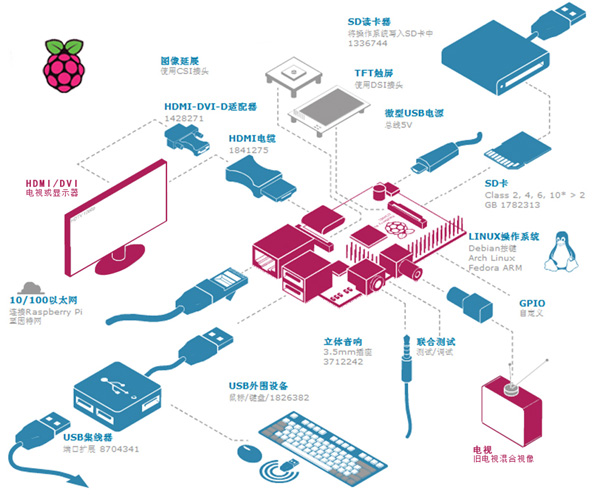
\includegraphics[width=0.7\linewidth]{Figure/rasp_all}
	\caption{树莓派基本硬件接口}
	\label{fig:rasp_1}
\end{figure}

如图\ref{fig:rasp_1}所示,树莓派包含的接口很多,包括USB电源接口、SD卡接口、GPIO、$I^{2}C$、USB2.0接口、CSI-2接口、HDMI接口、SVideo接口、以太网接口、3.5mm音频接口等。更可以通过USB接口连接分线器和鼠标键盘摄像头等实现扩展功能\cite{IoT}。

CSI属于MIPI标准之下。MIPI是一个比较新的标准,其规范也在不断修改和改进,目前比较成熟的接口应用有DSI(显示接口)和CSI(摄像头接口)。CSI/DSI分别是指其承载的是针对Camera或Display应用,都有复杂的协议结构。
CSI-2是一个单或双向差分串行界面,包含时钟和数据信号。CSI-2的层次结构:CSI-2由应用层、协议层、物理层组成。
由于串行接口一般采用差分结构,利用几百mV的差分信号,在收发端之间传送数据。串行比并行相比:更节省PCB板的布线面积,增强空间利用率;差分信号增强了自身的EMI抗干扰能力,同时减少了对其他信号的干扰;低的电压摆幅可以做到更高的速度,更小的功耗。

USB是连接电脑系统与外部设备的一种串口总线标准,也是一种输入输出接口的技术规范,被广泛地应用于个人电脑和移动设备等信息通讯产品,并扩展至摄影器材、数字电视(机顶盒)、游戏机等其它相关领域。目前含有多种型号。

以太网(Ethernet)是一种电脑局域网技术。IEEE组织的IEEE 802.3标准制定了以太网的技术标准,它规定了包括物理层的连线、电子信号和介质访问层协议的内容。以太网是目前应用最普遍的局域网技术,取代了其他局域网标准如令牌环、 FDDI 和 ARCNET 。这里用来连接互联网。

高清多媒体界面是(HDMI)一种全数字化影像和声音发送接口,可以发送未压缩的音频及视讯信号。HDMI可以同时发送音频和视讯信号,由于音频和视讯信号采用同一条线材,大大简化系统线路的安装难度。通过HDMI接口方便的连接到显示器进行图像显示。



\section{系统平台选择搭建}
%B/S(Browser/Server)架构,是浏览器和服务器的通信连接模式。在这一结构下,用户通过浏览器完成绝大多数的显示和回调,数据处理和归档还是主要通过服务器实现。这样可以大大简化的任务,减轻了系统维护与升级的成本,为用户的使用带来方便。但是,该方案有着系统运行速度和稳定性不够高的局限性。
%C/S(Client/Server)架构,即客户机和服务器的通信连接模式。它属于应用软件系统,充分利用客户端和服务器端的硬件环境,具体的运算和数据的处理被放在客户端,从而使客户端变得很“胖”,一般称为“胖客户机”;相对地,服务器端的任务较轻,称为“瘦服务器”,这样将任务合理分配到Client端和Server端来实现,降低了系统的通讯开销。
常见的架构方式包括B/S架构和C/S架构。B/S架构,是浏览器和服务器的通信连接模式。在这一结构下,用户通过浏览器完成绝大多数的显示和回调,数据处理和归档还是主要通过服务器实现。这样可以大大简化的任务,减轻了系统维护与升级的成本,为用户的使用带来方便。但是,考虑到网络的时延等,该方案有着系统运行速度和稳定性不够高的局限性。
\begin{figure}[h]
\centering
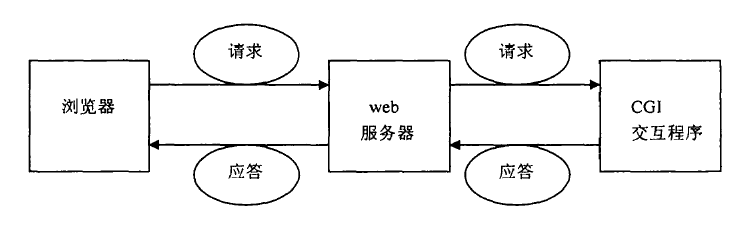
\includegraphics[width=0.7\linewidth]{Figure/bs01}
\caption{B/S架构图示}
\label{fig:bs01}
\end{figure}


C/S架构,即客户机和服务器的通信连接模式。它属于应用软件系统,充分利用客户端和服务器端的硬件环境,较为常见的是将具体的运算和数据的处理被放在客户端,从而使客户端变得很“胖”,一般称为“胖客户机”;相对地,服务器端的任务较轻,称为“瘦服务器”,和操作系统的连接较为紧密\cite{bscs}。
\begin{figure}[h]
\centering
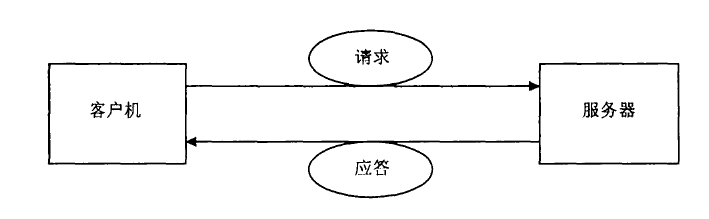
\includegraphics[width=0.7\linewidth]{Figure/cs01}
\caption{C/S架构图示}
\label{fig:cs01}
\end{figure}

相对于C/S模式,B/S模式显著的特点是浏览的跨平台操作,方便使用,考虑到跨平台的优势,所以目前越来越多的平台功能特性放在B/S架构下\cite{bshome}。
